\documentclass[english]{article}
\usepackage[T1]{fontenc}
\usepackage[utf8]{inputenc}
\usepackage[italian]{babel}
\usepackage{graphicx}
\usepackage{subcaption}
\usepackage{caption}
\usepackage{gensymb}
\usepackage{colortbl}
\usepackage{multicol}
\usepackage{wrapfig}

\usepackage{amsmath,bm}
\usepackage{siunitx}
\usepackage{float}
\usepackage{hyperref}
\captionsetup{tableposition=top,figureposition=bottom,font=footnotesize}
\renewcommand{\vec}{\mathbf}
\usepackage{upgreek}
\usepackage[a4paper, total={7in, 10in}]{geometry}
\begin{document}
\title{TITOLO:RELAZIONE DI DATA MINING}
\author{Daniele Maria Di Nosse, Angelo Lasala, Raffaele Paradiso}
\date{21/11/2020\newpage}

\maketitle
\tableofcontents{}

\newpage

\section{Introduzione}
Determinare le possibili relazioni che intercorrono fra caratteristiche dei dipendenti di un'azienda può risultare di grande utilità per predire i possibili scenari lavorativi che posso verificarsi e gestire di conseguenza l'organizzazione del personale in maniera ottimale. Nel presente progetto ci si pone l'obiettivo di valutare tali legami tramite un approccio di data mining. Le informazioni che si sono utilizzate sono relative ad un data frame fittizio (leggermente modificato) generato da IBM e presente sul portale Kaggle(URL \url{https://www.kaggle.com/pavansubhasht/ibm-hr-analytics-attrition-dataset}). Non ci si è posto un obiettivo principale, ovvero la determinazione di legami, correlazioni e classificazioni relativi ad un singolo attributo rispetto a tutti gli altri, ma si è proceduto in maniera più generale ricoprendo uno spettro più ampio di possibili relazioni fra tutte le variabili.

Sebbene i dati a disposizione siano stati divisi in due sotto insiemi, uno di Train ed uno di Test, si è deciso di utilizzare l'intero insieme di records per tutti i tasks che non concernono algoritmi di Machine Learning
\section{Data Understanding}
\subsection{Data Semantics}
Nella prima fase dell'elaborazione si è studiato il data frame nella sua forma originale (Train + Test), valutando il numero degli attributi, la loro natura e dominio. 

\begin{center}
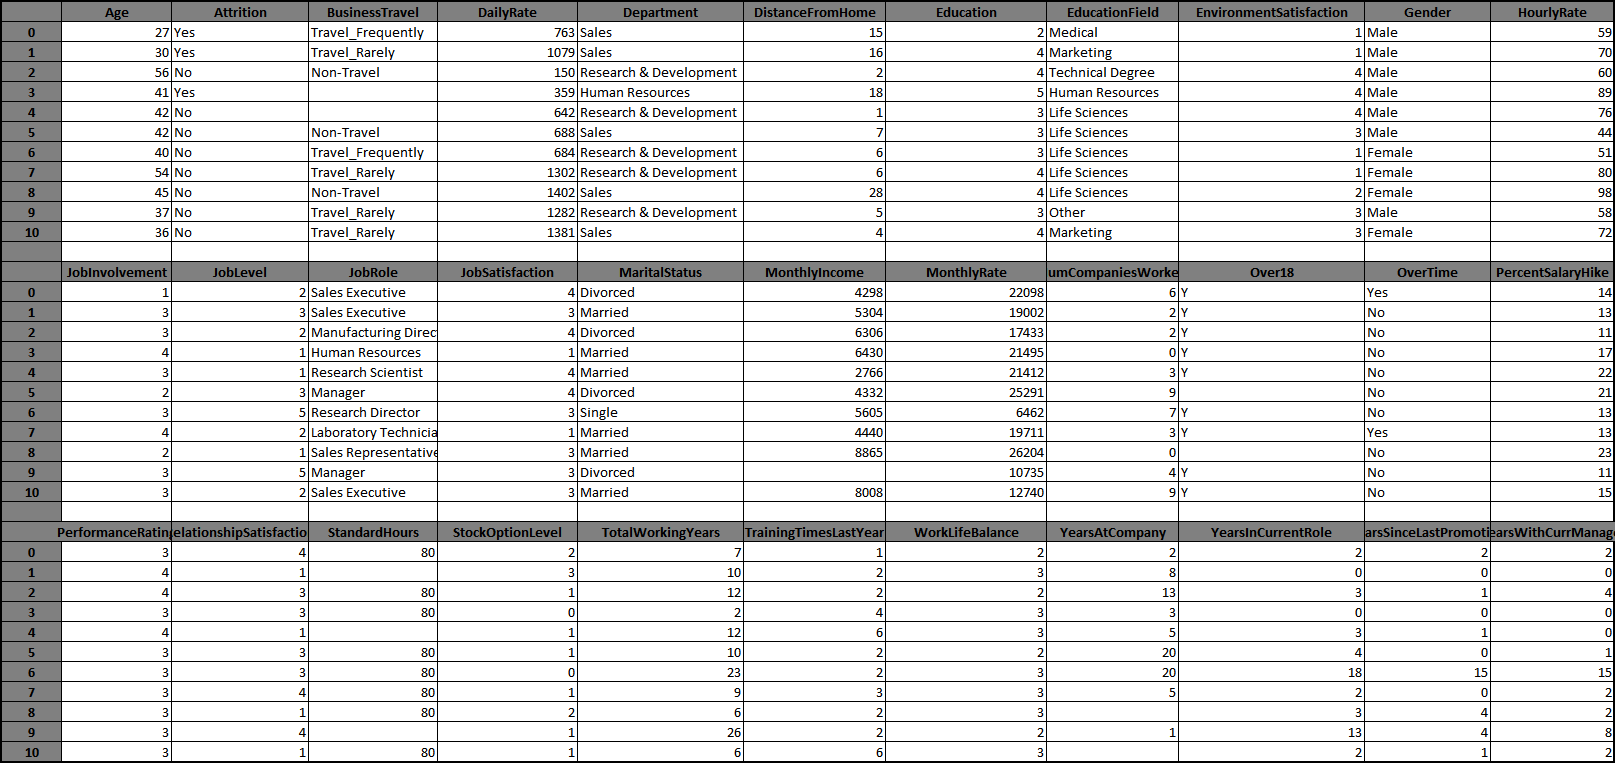
\includegraphics[scale=0.5]{DFhead(10).png}
\captionof{figure}{Primi 10 valori di ogni attributo}
\end{center}
% trim=2cm 0 0 0cm

Come si può notare dalla tabella precedente, il numero di attributi è pari a 33. Si dividono in attributi numerici e categorici, ma ad uno sguardo più attento si nota che alcuni di essi, come, ad esempio, Education o Enviroment Satisfaction, presentano valori numerici che poco si adattano al loro significato. Si ha infatti che sussistono le seguenti uguaglianze 

\begin{center}
\begin{tabular}{|c|c|c|c|c|c|c|}
\arrayrulecolor{white}\hline
Education & EnvironmentSatisfaction & JobInvolvement & JobSatisfaction \\
\arrayrulecolor{white}\hline
1 : 'Below College' & 1 : 'Low'  & 1 : 'Low'& 1 : 'Low' \\
2 : 'College'  & 2 : 'Medium' & 2 : 'Medium'& 2 : 'Medium'\\
3 : 'Bachelor'    &3 : 'High' & 3 : 'High'& 3 : 'High'  \\
4 : 'Master'    &4 : 'Very High' & 4 : 'Very High' & 4 : 'Very High' \\
5 : 'Doctor'  &  & &\\
\hline
\end{tabular}
\end{center}


%\begin{table}{I}{0.7\linewidth}
%\centering
\begin{center}
\begin{tabular}{|c|c|c|c|c|c|}
\arrayrulecolor{white}\hline
PerformanceRating & RelationshipSatisfaction&WorkLifeBalance  &   \quad\quad&\quad\quad    &\quad\quad      \\
\arrayrulecolor{white}\hline
1 : `Low' & 1 : `Low' & 1 : `Bad'&&&\\
2 : `Good' & 2 : 'Medium'& 2 : `Good'&&&\\
3 : `Excellent'& 3 : 'High' & 3 : `Better'&&&\\
4 : `Outstanding'& 4 : 'Very High' &4 : `Best'&&&\\
\hline
\end{tabular}
\end{center}

%\end{table}

Di conseguenza, il dominio di tali attributi è di tipo categorico od ordinale e non numerico(un attributo ordinale è effettivamente una sottocategoria categorica. Si è scelto comunque di elencarli separatamente). Inoltre, sebbene non si abbiano informazioni dettagliate sulle classi relative agli attributi JobLevel e  StockOptionLevel, per la loro stessa natura si è deciso di trattarli come attributi ordinali. Organizzando tutte le variabili per la loro tipologia, si ottiene quindi che

\begin{center}
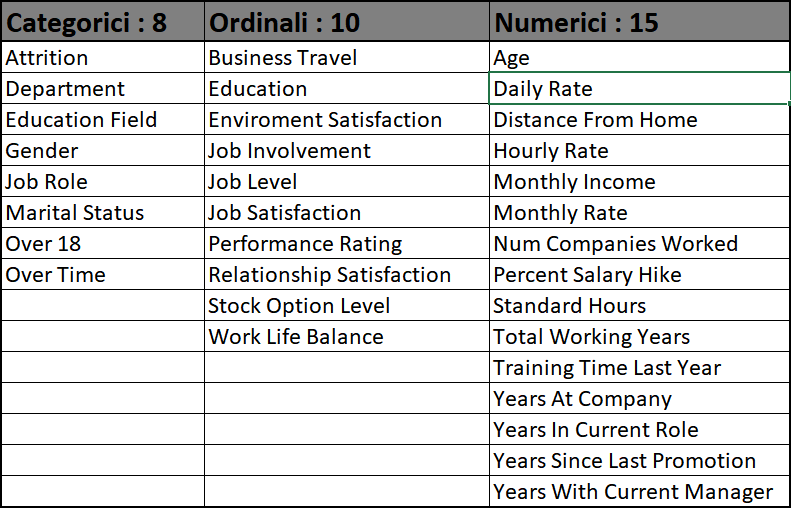
\includegraphics[scale=0.50]{semantics.png}
\captionof{figure}{Domini degli attributi}
\end{center}
Per quanto riguarda il range di valori degli attributi risulta essere molto più discretizzato per gli attributi ordinali che per gli attributi numerici. Inoltre differisce molto da attributo ad attributo (anche di 4 ordini di grandezza), cosa che sottolinea sin da questo punto l'importanza di una trasformazione delle variabili.

\subsection{Analisi statistica}
Le frequenze degli attributi categorici e le relative mode sono riportate nelle seguenti tabelle

\begin{center}
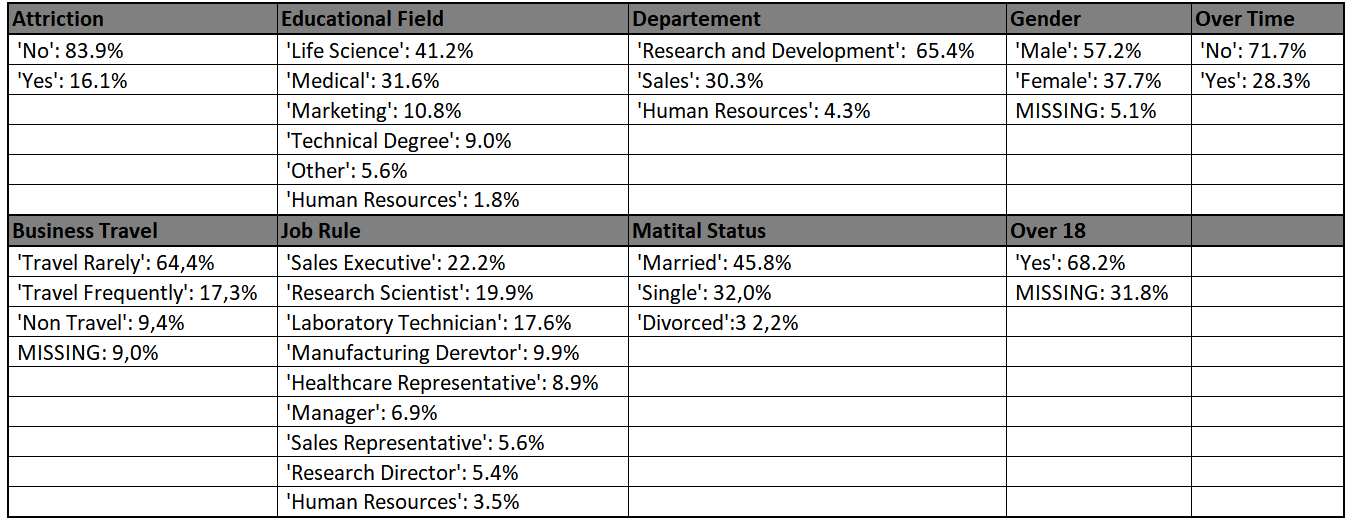
\includegraphics[scale=1.28]{frequenza attributi nominali.png}
\captionof{figure}{Frequenze degli attributi categorici}
\end{center}

\begin{center}
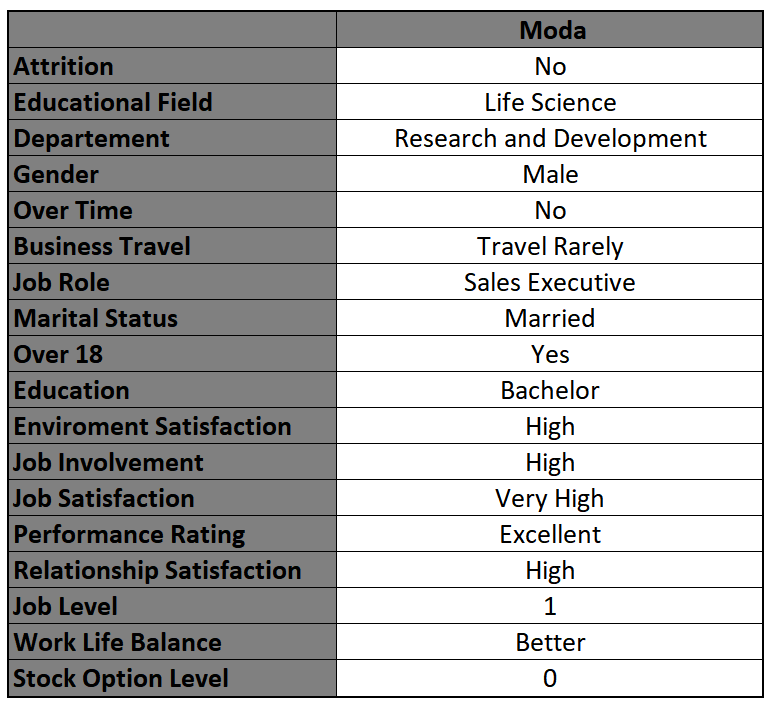
\includegraphics[scale=1.28]{modacategoriciordinali.png}
\captionof{figure}{Mode}
\end{center}
 
 
mentre le distribuzioni degli attributi ordinali e numerici con alcuni indici statistici sono rappresentate di seguito.
Si può notare la forte asimmetria di molte distribuzioni ed un varianza molto grande in alcuni attributi. Tali problematiche dovranno essere sanate con opportune trasformazioni.

\begin{center}
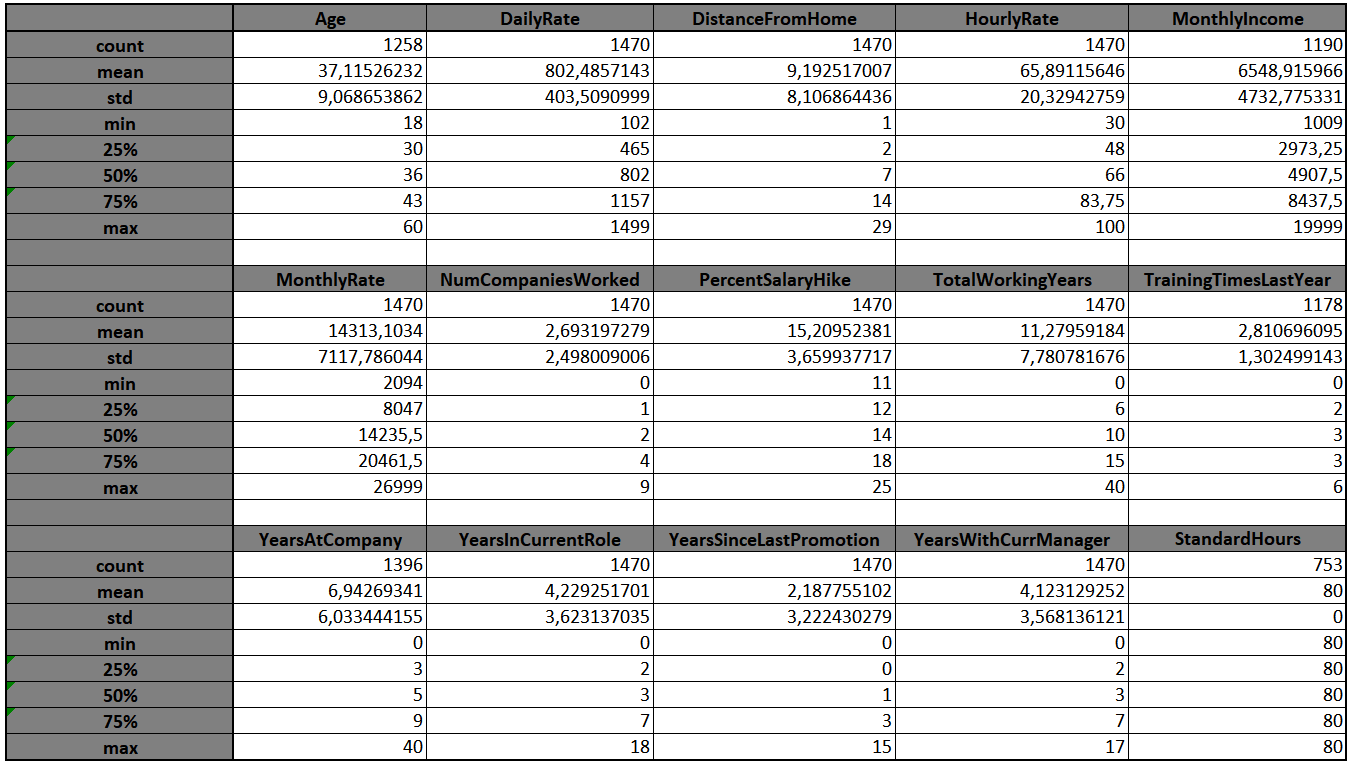
\includegraphics[scale=1.3]{statistica.png}
\captionof{figure}{Indici statistici per gli attributi numerici}
\end{center}

\begin{center}
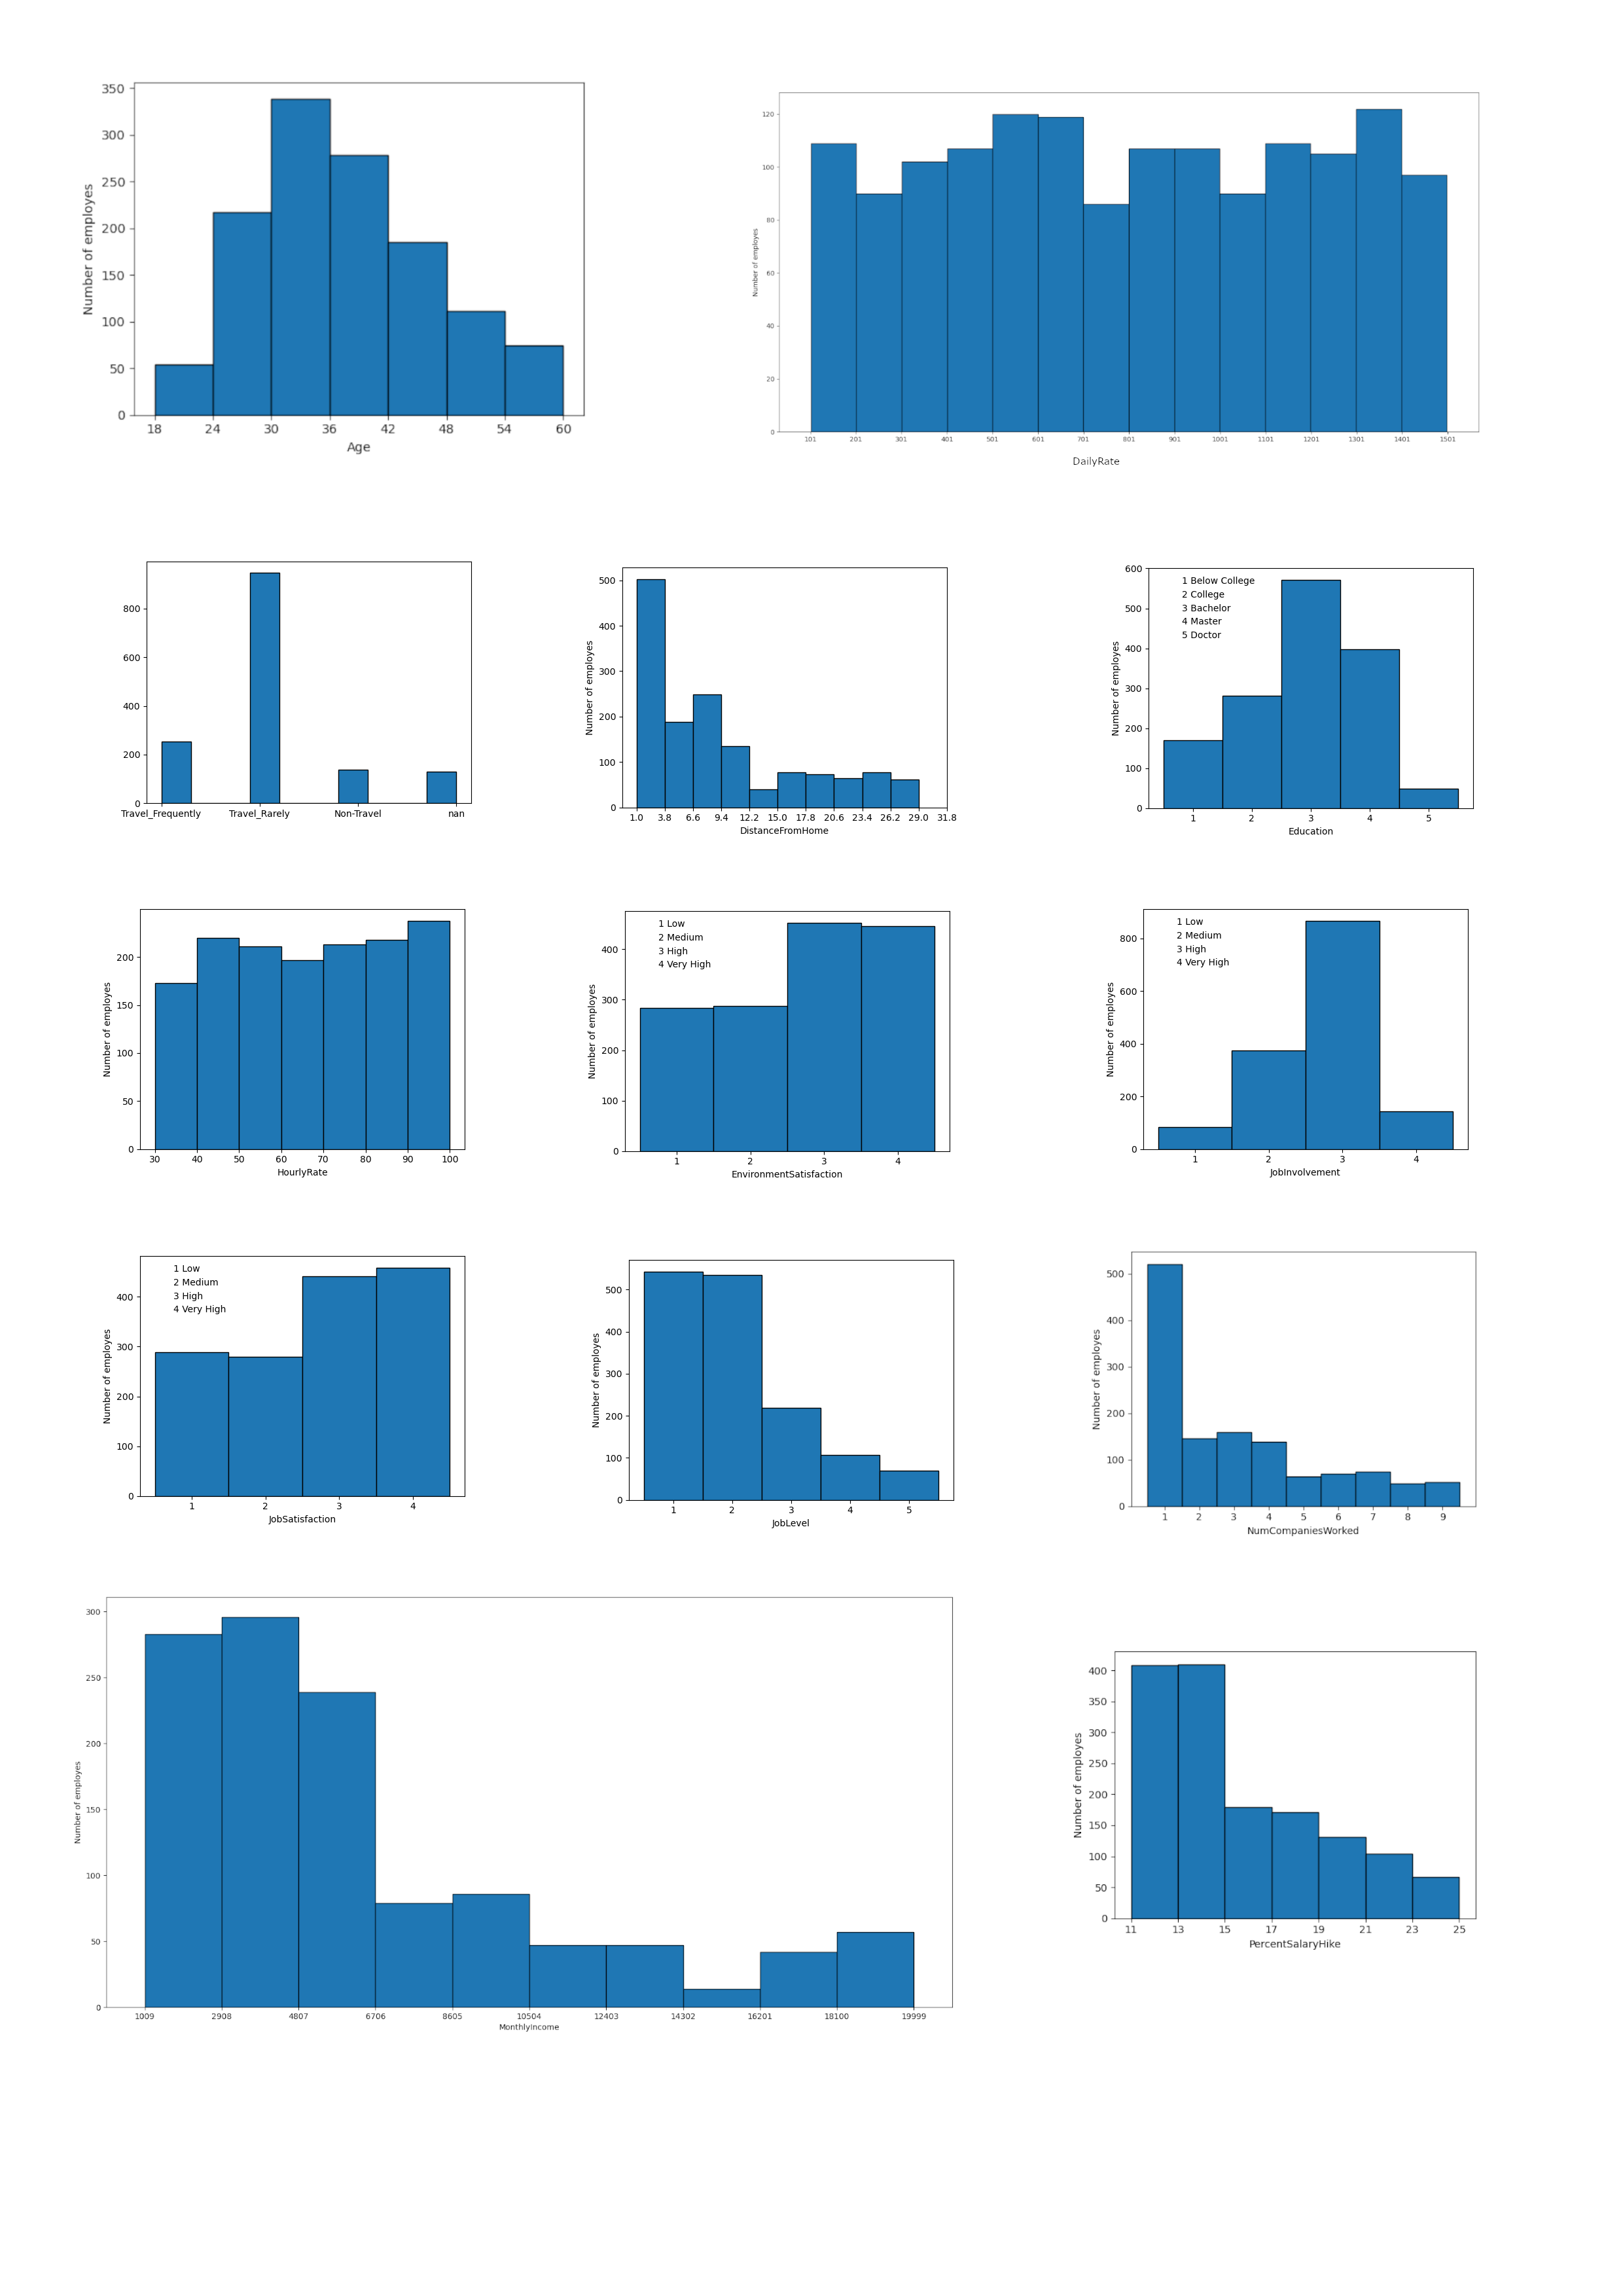
\includegraphics[scale=0.9,trim=0.5cm 0 0 0cm]{Istogrammi1.png}
\end{center}

\begin{center}
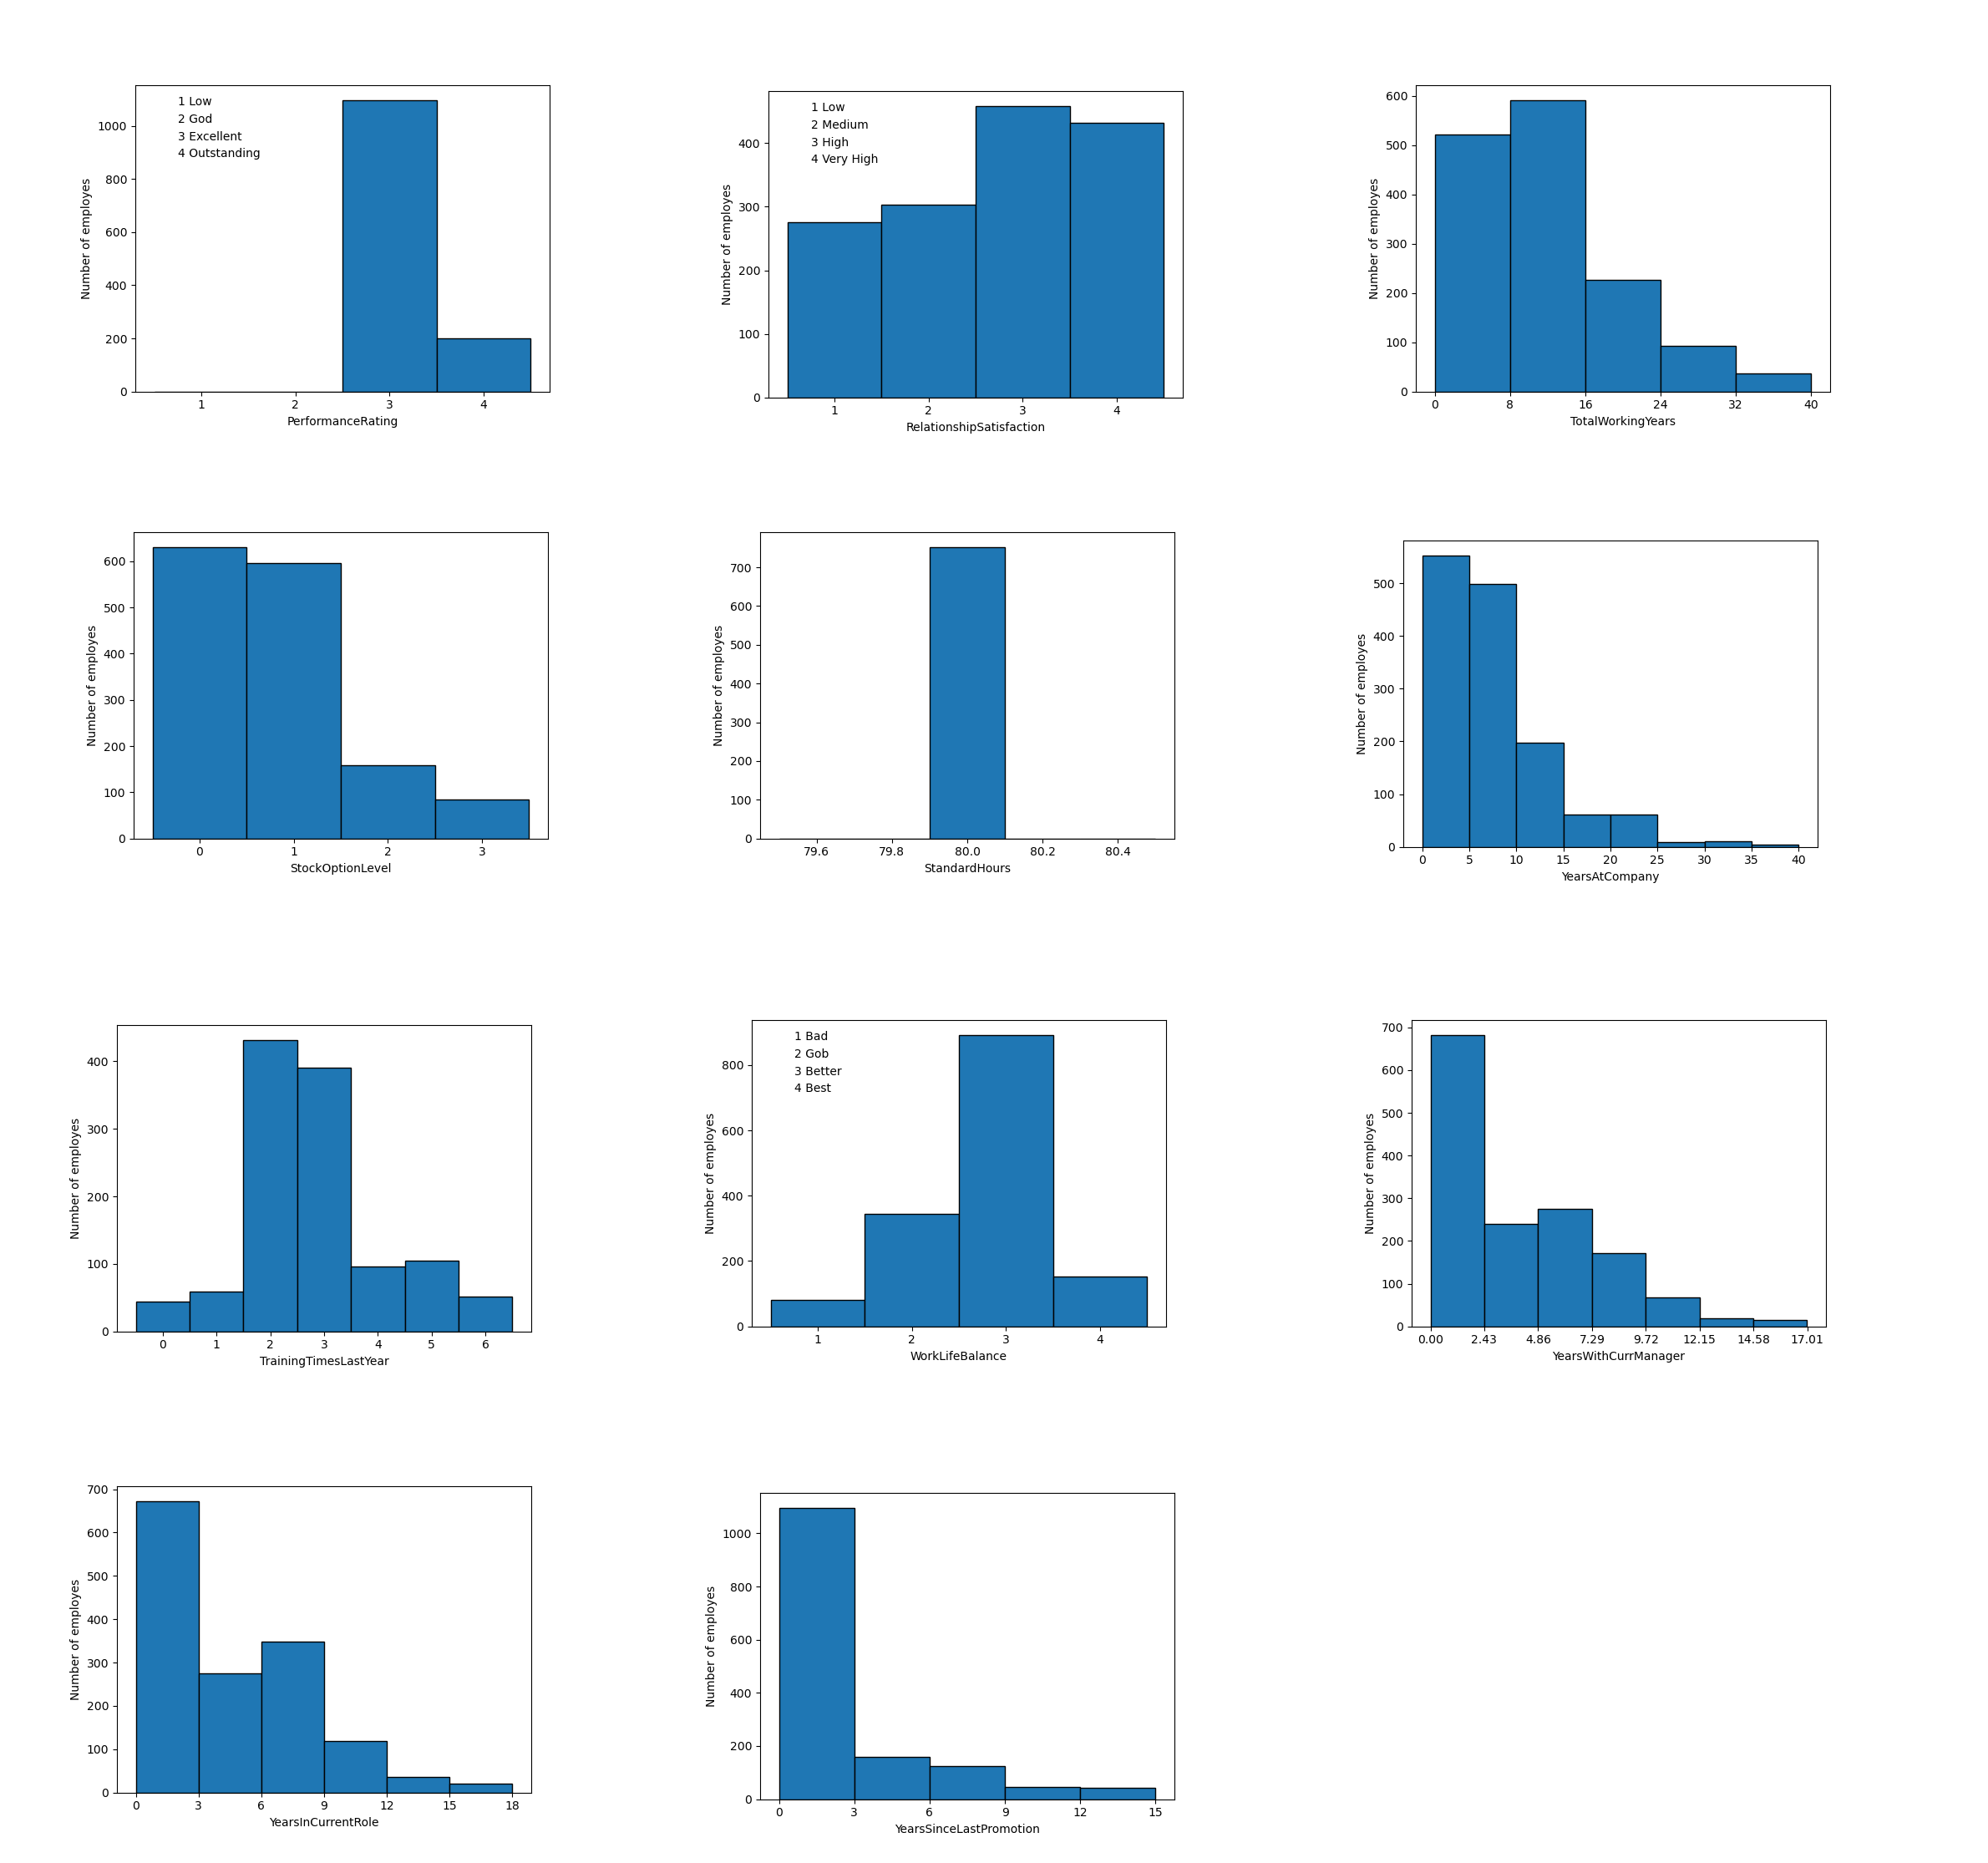
\includegraphics[scale=1,trim=1cm 0 0 0cm]{Istogrammi2.png}
\captionof{figure}{Istogrammi attributi numerici ed ordinali}
\end{center}

\subsection{Data Quality : Outliers e Missing values}
La qualità dei dati è fortemente influenzata, negativamente, dalla presenza di outliers e di missing values. Algoritmi di clustering e correlazioni fra gli attributi possono restituire risultati falsificati se non si gestiscono in maniera appropriata tali valori. 
Nel data frame utilizzato la loro presenza è evidente, infatti

\begin{center}
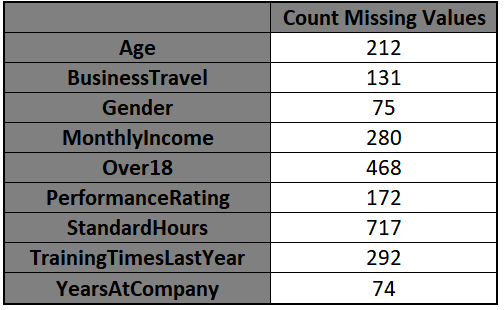
\includegraphics[scale=1]{missingvalues.png}
\captionof{figure}{Count dei missing values}
\end{center}
Gli attributi StandardHours ed Over18 presentano una qualità molto scarsa: nel primo circa la metà dei records sono mancanti e la restante parte ha un unico valore, mentre il secondo, oltre a contenere anch'esso una quantità significativa di missing values, non rappresenta in ogni caso un attributo di grande importanza, considerando che la stragrande maggioranza dei dipendenti di un'azienda sono maggiorenni. Per tali motivi, si è deciso di eliminare questi due attributi.

Per la determinazione degli outliers si sono valutati sia test puramente statistici (Grubbs's test) che metodi di visualizzazione (Box Plot e Principal Component Analysis). Come è noto, per utilizzare approcci del primo tipo bisogna fare delle assunzioni sulla distribuzione sottostante dei valori esaminati. In particolare, il Grubbs's test, applicabile singolarmente agli attributi, richiede che i dati siano distribuiti normalmente, cosa non vera in questo caso. Di conseguenza, tale metodo è stato scartato. 
Il Principal Component Analysis, d'altro canto, è uno dei metodi maggiormente utilizzati nella ricerca di outliers in situazioni alto-dimensionali. Proiettando lo spazio n-dimensionale in uno spazio q-dimensionale ($q<n$) costruito tramite i vettori normalizzati della matrice di correlazione, si cerca di mantenere il più intatta possibile la varianza negli attributi. Nel caso in esame, la frazione di varianza conservata non risulta essere significativa (circa $0.4$), inficiando inevitabilmente i risultati ottenuti.
L'unico metodo che ha avuto successo per la determinazione degli outliers è stata la visualizzazione dei Box Plot per i singoli attributi. Si è proceduto quindi alla loro rimozione tramite eliminazione delle righe corrispondenti.

\section{Data Preparation}
In questa fase del lavoro ci si è posto l'obiettivo di trasformare e preparare il set di dati all'analisi successiva. I problemi precedentemente evidenziati sono stati qui risolti.\\

Come primo task sono stati gestiti i missing values.\\
Nell'attributo BusinessTravel presenta una frequenza di NaN pari al circa $9\%$, confrontabile con le frequenze degli altri valori . Siccome la granulosità dell'attributo ricopre in maniera completa lo spettro delle classi plausibilmente ad esso associabili, si è deciso di valutare se ci fosse dipendenza con gli altri attributi presenti nel data frame. Per quanto riguarda quella con gli numerici, sono stati utilizzati gli scatter plot, mentre per quelli nominali è stato eseguito il test di indipendenza del chi quadro. In entrambi i casi non si sono evinte dipendenze significative ($p value $>$ 0.05$ sempre). Di conseguenza tale attributo è stato scartato.\\

Per quanto riguarda PerformanceRating, si è aggiunta una nuova classe 'MISSING', poiché si è notato che la granulosità dell'attributo non ricopre tutto lo spettro plausibile. Si presuppone che i valori MISSING possano appartenere ad una classe di ordine inferiore ad Excellent.\\

Queste due considerazioni non sono applicabile all'attributo Gender per il quale si è scelto semplicemente di sostituire ai missing values valori estratti dalla distibuzione nota.\\

Procedimento analogo è stato applicato a tutti gli attributi numerici che presentano valori mancanti, l'unica differenza è che in questo caso i valori sostitutivi sono le medie degli intervalli dei bins degli istogrammi.\\ %(che al mercato mio padre comprò, nda).\\

Il metodo di visualizzazione grafica dei Box Plot evidenzia la presenza di outliers solo in tre attributi numerici: TreningTimeLastYear, TotalWorkingYears, YearsAtCompany
\begin{center}
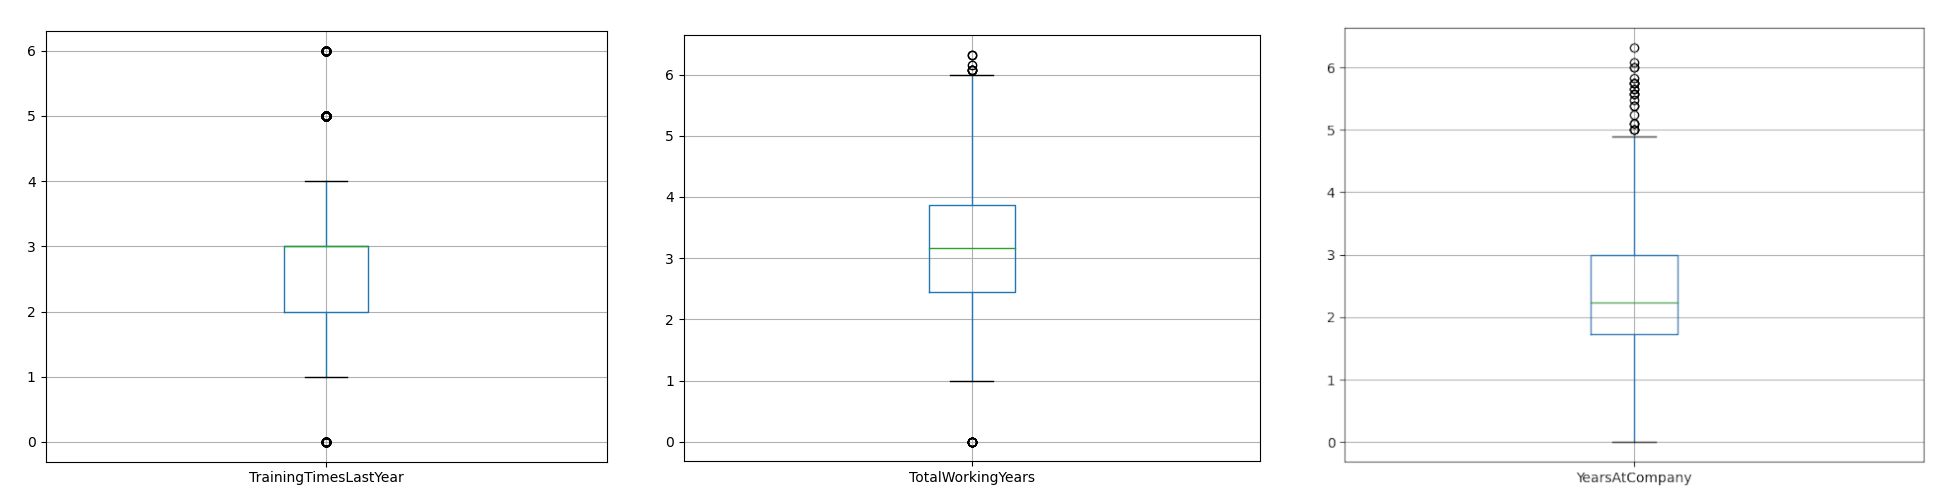
\includegraphics[scale=1]{boxplot.png}
\captionof{figure}{Box Plot degli attributi che presentano outliers}
\end{center}
 Il data freme  dopo questa prima preparazione risulta contienere il $36\%$ di dati in meno rispetto a quello di partenza.\\

Funzioni di trasformazione sono state applicate ad attributi numerici con lo scopo di rimediare ad alcune caratteristiche delle loro distribuzioni quali l'asimettrie e un valore spropositato della deviazione standar. In particolre è stata applicata la radice quadrata ad DistanceFromHome, NumCompaniesWorked, PercentSalaryHike, TotalWorkingYears, YearsAtCompany, YearsInCurrentRole, YearsSinceLastPromotion e YearsWithCurrManager; invece ad MonthlyIncome è stato applicato il logaritmo naturale. Di seguito sono riportate alcune distribuzione delle variabili trasformate.

\section{Clustering}

\section{Conclusioni}
\end{document}
